\documentclass{article}

\usepackage{amsmath}
\usepackage{minted}
\usepackage[ruled,vlined]{algorithm2e}
\usepackage[utf8]{inputenc}
\usepackage[english]{babel}
\usepackage{blindtext}
\usepackage{amssymb}
\usepackage{scrextend}
\usepackage{multicol}
\usepackage{wrapfig}
\usepackage{tikz}

\usepackage{amsthm}

\usepackage[margin=1in]{geometry}
\pagestyle{empty}

\title{\vspace{-3cm}Homework 2}
\author{Yutong Huang (yxh589)}
\date{}

\begin{document}
\pagenumbering{gobble}
\maketitle
\section*{Problem 1}
To prove this problem is equivalent to showing that a multicore TM can be simulated
by a single core, single tape TM. We can do this by showing that a single core, single
tape TM can simulate a single core, multitape TM, and then show that a single core multitape
machine can simulate a multicore multitape TM.
\begin{proof}
    Say MM is a multicore, multitape TM that has $k$ heads and $k$ tapes. Similarly,
    SM is a single head $k$ tape machine, and SS is a single head single tape mahcine.\\*

    Consider an arbitrary transition function on MM:
    $$\delta_{MM}((q_{1m^*}, q_{2m^*},\dots,q_{km^*}),(a_1, a_2,\dots, a_k))=((q_{1n^*}, q_{2n^*}, \dots, q_{kn^*}), (b_1, b_2,\dots, b_k), (L, R, L, \dots, R))$$

    where $q_{im^*}$ represents an arbitrary state on the i-th head before the transition, and $q_{jn^*}$
    represents the resulting state on the j-th head after the transition. Similarly, $a_i$ represents the value read at the i-th head before transition,
    and $b_j$ represents the value written to the j-th head. L, R, L, S \dots are movement directions for
    each head respectively.\\*

    This function can be simulated on SM with the following transition function:
    $$\delta_{SM}(q_{m1}, (a_1, a_2, \dots, a_k))=(q_{m2}, (b_1, a_2,\dots, a_k), (L, S, S, S,\dots))$$
    $$\delta_{SM}(q_{m2}, (b_1, a_2, \dots, a_k))=(q_{m3}, (b_1, b_2,\dots, a_k), (S, R, S, S,\dots))$$
    $$\dots$$
    $$\delta_{SM}(q_{mk}, (b_1, b_2, \dots, b_{k-1}, a_k))=(q_{n}, (b_1, b_2,\dots, b_k), (S, S, S, S,\dots), (S, S, S,\dots, R))$$

    Therefore, any arbitrary transition function on MM can be simulated on SM.\\*

    Similarly, consider an arbitrary transition function on a SM:
    $$\delta_{SM}(q_m, (a_1, a_2, \dots, a_k))=(q_n, (b_1, b_2,\dots, b_k), (L,R, \dots, L))$$

    On SS, we can use a special character such as $\#$ to seperate the tape in to multiple
    segments, representing multiple tapes. Then we can use an asterisk(*) to mark the cell that
    this simulated head is currently pointing at. Next we can construct a transition function as follows:\\*
    % $w_{11}^*, w_{12},\dots,\#, w_{21}, w_{22}^*,...,\#\dots\#, w_{k1},w_{k2},\dots, w_{kn}^*, \dots$

    SS: on input=$ w_1, w_2,\dots, w_n$
    \begin{enumerate}
        \item the input format would be $\#w_1^* w_2 w_3 \dots w_n \# \_^* \# \_^* \# \dots \#$, which simulates k tapes.
        \item SS scans the tape from the first \# to the (k+1)-th \# (which is essentially a left end to right end sweep) to
              determine the value at each simulated heads (cells marked with a *).
        \item then the machine sweeps throught the tape again to update values as described in
              SM's transition function.
        \item if one of the heads shifts right to a \#, then SM writes a $\_^*$ in its place and shift the content to the right
              of the \# (including the \#) to the right by 1 cell.
        \item go back to step 2 and continue the simulation.
    \end{enumerate}

    Therefore, any arbitrary transition function of SM can be simulated on SS.

    Any arbitrary transition function of SM can be simulated on SS $\land$ any arbitrary transition function on MM can be simulated on SM
    $\implies$ SS can simulate all transition functions on SM that simulate MM \\*
    $\implies$ SS can simulate any arbitrary transition function on MM.

\end{proof}
\newpage
\section*{Problem 2}

To show that this machine can recognize all languages recognizable by a normal TM, we just need to show that we can
emulate a left move on this broken machine. Below is a diagram that describes a procedure that
move one cell to the left. 


\begin{center}
    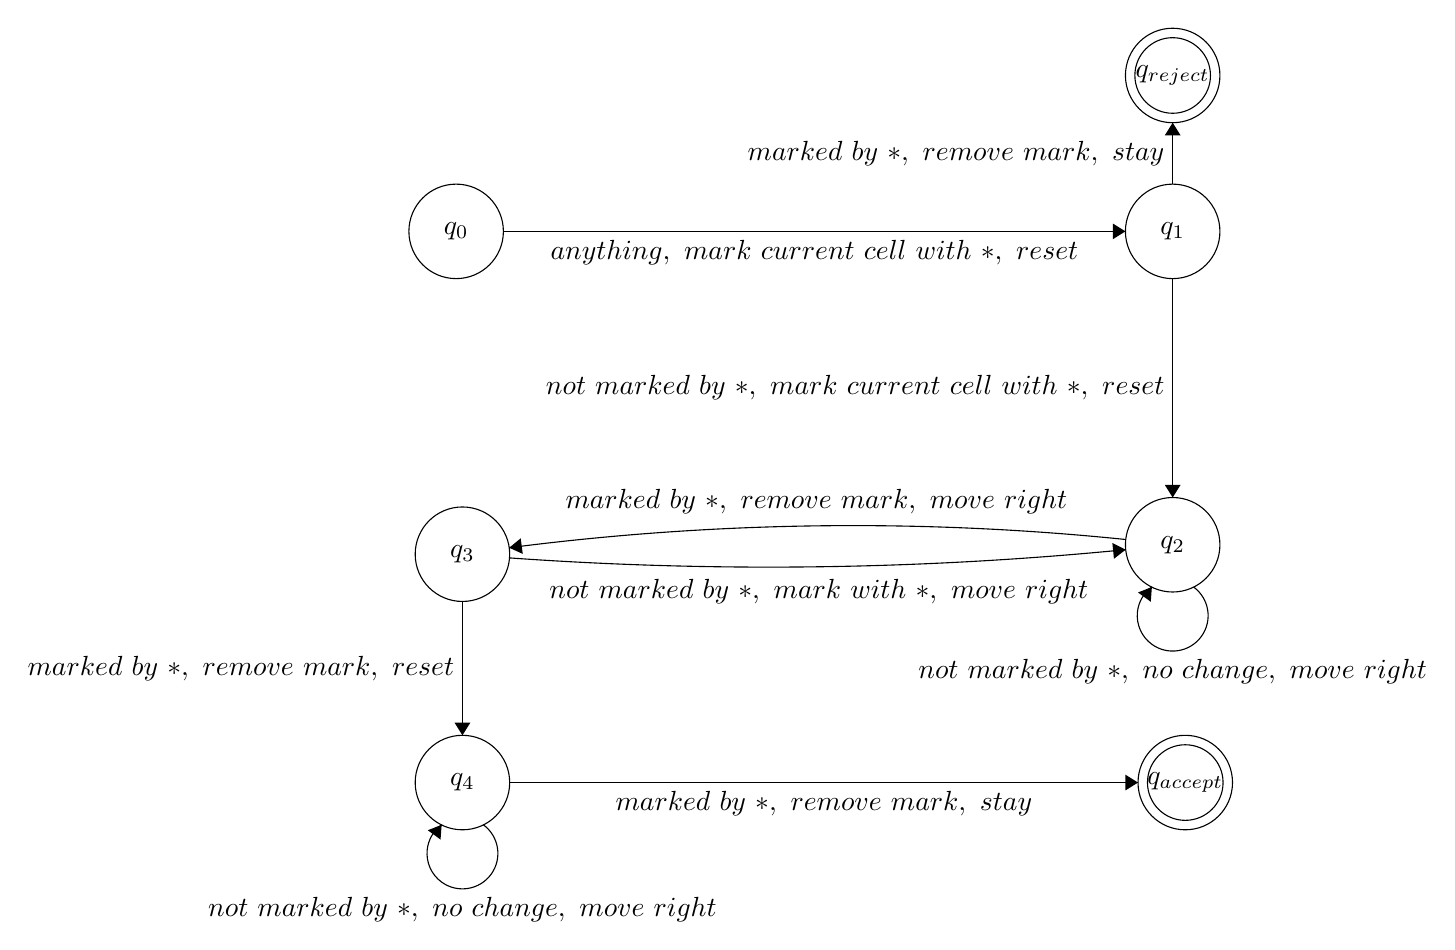
\begin{tikzpicture}[scale=0.2]
        \tikzstyle{every node}+=[inner sep=0pt]
        \draw [black] (12.3,-12.7) circle (3);
        \draw (12.3,-12.7) node {$q_0$};
        \draw [black] (57.8,-12.7) circle (3);
        \draw (57.8,-12.7) node {$q_1$};
        \draw [black] (57.8,-32.6) circle (3);
        \draw (57.8,-32.6) node {$q_2$};
        \draw [black] (12.7,-33.2) circle (3);
        \draw (12.7,-33.2) node {$q_3$};
        \draw [black] (12.7,-47.7) circle (3);
        \draw (12.7,-47.7) node {$q_4$};
        \draw [black] (58.6,-47.7) circle (3);
        \draw (58.6,-47.7) node {$q_{accept}$};
        \draw [black] (58.6,-47.7) circle (2.4);
        \draw [black] (57.8,-2.8) circle (3);
        \draw (57.8,-2.8) node {$q_{reject}$};
        \draw [black] (57.8,-2.8) circle (2.4);
        \draw [black] (15.3,-12.7) -- (54.8,-12.7);
        \fill [black] (54.8,-12.7) -- (54,-12.2) -- (54,-13.2);
        \draw (35.05,-13.2) node [below] {$anything,\mbox{ }mark\mbox{ }current\mbox{ }cell\mbox{ }with\mbox{ }*,\mbox{ }reset$};
        \draw [black] (57.8,-15.7) -- (57.8,-29.6);
        \fill [black] (57.8,-29.6) -- (58.3,-28.8) -- (57.3,-28.8);
        \draw (57.3,-22.65) node [left] {$not\mbox{ }marked\mbox{ }by\mbox{ }*,\mbox{ }mark\mbox{ }current\mbox{ }cell\mbox{ }with\mbox{ }*,\mbox{ }reset$};
        \draw [black] (15.672,-32.789) arc (97.37052:84.15389:170.098);
        \fill [black] (15.67,-32.79) -- (16.53,-33.18) -- (16.4,-32.19);
        \draw (35.17,-30.68) node [above] {$marked\mbox{ }by\mbox{ }*,\mbox{ }remove\mbox{ }mark,\mbox{ }move\mbox{ }right$};
        \draw [black] (59.123,-35.28) arc (54:-234:2.25);
        \draw (57.8,-39.85) node [below] {$not\mbox{ }marked\mbox{ }by\mbox{ }*,\mbox{ }no\mbox{ }change,\mbox{ }move\mbox{ }right$};
        \fill [black] (56.48,-35.28) -- (55.6,-35.63) -- (56.41,-36.22);
        \draw [black] (54.816,-32.912) arc (-84.39444:-94.08115:231.718);
        \fill [black] (54.82,-32.91) -- (53.97,-32.49) -- (54.07,-33.49);
        \draw (35.33,-34.73) node [below] {$not\mbox{ }marked\mbox{ }by\mbox{ }*,\mbox{ }mark\mbox{ }with\mbox{ }*,\mbox{ }move\mbox{ }right$};
        \draw [black] (12.7,-36.2) -- (12.7,-44.7);
        \fill [black] (12.7,-44.7) -- (13.2,-43.9) -- (12.2,-43.9);
        \draw (12.2,-40.45) node [left] {$marked\mbox{ }by\mbox{ }*,\mbox{ }remove\mbox{ }mark,\mbox{ }reset$};
        \draw [black] (14.023,-50.38) arc (54:-234:2.25);
        \draw (12.7,-54.95) node [below] {$not\mbox{ }marked\mbox{ }by\mbox{ }*,\mbox{ }no\mbox{ }change,\mbox{ }move\mbox{ }right$};
        \fill [black] (11.38,-50.38) -- (10.5,-50.73) -- (11.31,-51.32);
        \draw [black] (15.7,-47.7) -- (55.6,-47.7);
        \fill [black] (55.6,-47.7) -- (54.8,-47.2) -- (54.8,-48.2);
        \draw (35.65,-48.2) node [below] {$marked\mbox{ }by\mbox{ }*,\mbox{ }remove\mbox{ }mark,\mbox{ }stay$};
        \draw [black] (57.8,-9.7) -- (57.8,-5.8);
        \fill [black] (57.8,-5.8) -- (57.3,-6.6) -- (58.3,-6.6);
        \draw (57.3,-7.75) node [left] {$marked\mbox{ }by\mbox{ }*,\mbox{ }remove\mbox{ }mark,\mbox{ }stay$};
    \end{tikzpicture}
\end{center}

This procedure will find the cell to the left of current cell if current cell is not the leftmost cell, otherwise the procedure would reject and stay in place.

\begin{proof}
    Assume an arbitrary language $L$ is recognized by a normal TM.\\*
    $\implies \exists M$ that recognizes $L$. \\*

    Consider an algorithm $M'$ which is exactly identical to $M$ except that every left move is replaced by 
    the above procedure. Then $M'$ also recognizes $L$.\\*

    Therefore, any language recognizable to a normal TM is also recognizable to this broken machine.\\*
\end{proof}


\section*{Problem 3}
(a)
\begin{proof}
    Assume $L_1$ and $L_2$ are decidable $\implies$ $\exists M_1, M_2$ that decides $L_1$ and $L_2$ respectively.\\*

    Consider an arbitrary language $l=ab$, and the 
    following algorithm:
    \begin{algorithm}
        \caption{M}
        \SetKwInOut{Input}{Input}
        \DontPrintSemicolon
        \Input{ab}
        Run $M_1$ on a\;
        \If{$M_1$ rejects}{
            \Return reject\;
        }
        Run $M_2$ on a\;
        \If{$M_2$ rejects}{
            \Return reject\;
        }
        \Return accept;
    \end{algorithm}\\*

    Case 1: $l \in L \implies a \in L_1 \land b \in L_2$:
    \begin{addmargin}[2em]{0em}
        Both $M_1$ and $M_2$ accepts; \\*
        $\implies$ M accepts;\\*
    \end{addmargin}

    Case 2: $l \notin L$:
    \begin{addmargin}[2em]{0em}
        Case 2.1: $a \notin L_1 \land b \in L_2$
        \begin{addmargin}[1em]{0em}
        $M_1$ rejects $\implies$ M rejects; 
        \end{addmargin}
        Case 2.2: $a \in L_1 \land b \notin L_2$
        \begin{addmargin}[1em]{0em}
        $M_2$ rejects $\implies$ M rejects;
        \end{addmargin}
        Case 2.3: $a \notin L_1 \land b \notin L_2$
        \begin{addmargin}[1em]{0em}
        Both $M_1$ and $M_2$ reject $\implies$ M rejects;\\*
        \end{addmargin}
    \end{addmargin}

    Therefore, M accepts if $l \in L$, rejects if $l \notin L \iff$ M decides L\\*
    
    $\implies$ L is decidable.
\end{proof}
(b)
\begin{proof}
    Assume $L_1$ and $L_2$ are recognizable $\implies$ $\exists M_1, M_2$ that recognize $L_1$ and $L_2$ respectively.\\*

    Consider the abouve algorithm again, and an arbitrary input $l=ab$\\*

    Case 1: $l \in L \implies a \in L_1 \land b \in L_2$:
    \begin{addmargin}[2em]{0em}
        Both $M_1$ and $M_2$ accepts; \\*
        $\implies$ M accepts;\\*
    \end{addmargin}

    Case 2: $l \notin L$:
    \begin{addmargin}[2em]{0em}
        Case 2.1: $a \notin L_1 \land b \in L_2$
        \begin{addmargin}[1em]{0em}
        $M_1$ rejects or infinite loop $\implies$ M rejects or infinite loop; 
        \end{addmargin}
        Case 2.2: $a \in L_1 \land b \notin L_2$
        \begin{addmargin}[1em]{0em}
        $M_2$ rejects or infinite loop $\implies$ M rejects or infinite loop;
        \end{addmargin}
        Case 2.3: $a \notin L_1 \land b \notin L_2$
        \begin{addmargin}[1em]{0em}
        Both $M_1$ and $M_2$ reject or infinite loop $\implies$ M rejects or infinite loop;\\*
        \end{addmargin}
    \end{addmargin}

    Therefore, M accepts if $l \in L$, M rejects or infinite loop if $l \notin L$ \\*
    $\iff$ M recognizes L $\iff$ L is recognizable.
\end{proof}
\end{document}